\documentclass[10pt,twocolumn,letterpaper]{article}
\usepackage[pagenumbers]{cvpr}
\usepackage[T1]{fontenc}
\usepackage{graphicx,booktabs,amsmath}
\usepackage[breaklinks,colorlinks,citecolor=blue,urlcolor=blue,linkcolor=blue]{hyperref}
\def\confName{NOWAI}
\def\confYear{2026}
\begin{document}
\title{One Prefill Prices a Pool of Reasoning Models\\Supplementary Material}
\author{Anonymous authors}
\maketitle

\section{Available and Captured Savings}
Figure~\ref{fig:headroom} reports the empirical oracle opportunity alongside learned savings. Headroom is defined relative to the same median-output reference, with success predictions held fixed. Each pool uses its own shared accuracy band. Contrast pools have different models and prices, so the comparison is descriptive. Oracle output lengths are estimated from repeated generations and have sampling error.
\begin{figure*}[t]
\centering
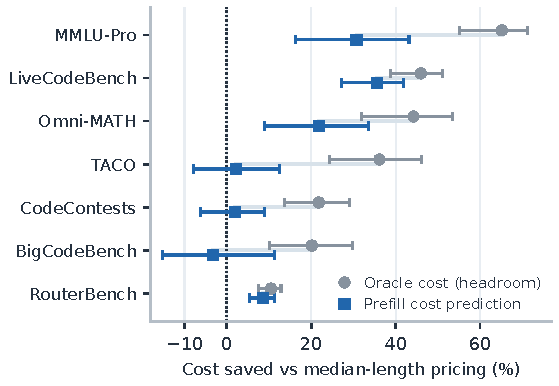
\includegraphics[width=.60\textwidth]{figures/headroom_and_capture.pdf}
\caption{Available savings can remain uncaptured. Oracle and predicted costs replace median output length with success predictions held fixed. Whiskers are paired 95\% problem-bootstrap intervals. Oracle headroom alone does not establish a learnable routing signal.}
\label{fig:headroom}
\end{figure*}

\section{Additional Controls and Baseline Scope}
A mean-output constant control substitutes mean training output length for the median. A query-independent model-mixture control constructs the convex hull of the fixed routes' observed cost and accuracy, allowing randomized mixtures. It is not a single best model. Reachable accuracy bands can differ; subtracting separately summarized gains does not directly measure savings at identical accuracy targets.

The embedding baseline averages MLP, random-forest and nearest-neighbor predictions from jina-code embeddings. The GBM uses prompt length, numbers, examples, constraints and keyword counts. These adapt estimator families rather than reproduce complete MixLLM or CARROT routers. Cost-from-success uses all routes' predicted success logits and squares, rather than one scalar difficulty. All fit training output lengths and use the dedicated head's price conversion.

The ZeroRouter comparison uses a MAP point estimate rather than hierarchical SVI. Frozen prefill features are reduced to 256 training-fitted PCA components and mapped to item parameters using ridge regression. Dimensions $\{1,5\}$, optimization seeds $\{0,1,2\}$ and bin counts $\{5,10,20\}$ are selected on calibration, with 1,500 Adam steps per IRT fit. The deployment pool has five routes rather than the original population-scale setting. Difficulty-bin controls and an alternative encoder implementation are secondary analyses, not equivalent implementations of the original system.

\section{Exploratory Cross-Fitting}
A subsequent five-fold analysis refitted both methods using training and calibration partitions excluding each outer test fold. Configuration selection remained inside calibration. Every problem received one held-out prediction.
\begin{table}[t]
\centering
\footnotesize
\begin{tabular}{lrr}
\toprule
Pool & $n$ & Difference [conditional interval] \\
\midrule
LiveCodeBench & 892 & $+$18.4 [14.1, 22.6] \\
Omni-MATH-500 & 500 & $+$13.8 [6.5, 21.6] \\
MMLU-Pro & 1,000 & $+$23.8 [12.5, 33.0] \\
\bottomrule
\end{tabular}
\caption{Ours minus calibration-selected ZeroRouter reimplementation, in percentage points of savings versus median pricing. Intervals are 95\% paired percentile bootstrap intervals conditional on fitted heads, omitting training variability.}
\end{table}

This uses one shuffled partition (seed 17), larger training fractions, and random rather than original splits; LiveCodeBench's original split is temporal. The 1,000-resample bootstrap fixes predictions and omits dependence from overlapping training sets. It does not establish three algorithm-level significant wins. Individual Omni fold effects range from $-4.2$ to $+30.2$ points. The original fixed-split comparison remains distinct.

On the original test sets, generation-resampling standard deviations are 1.72, 3.72 and 2.69 percentage points for LiveCodeBench, Omni and MMLU-Pro, versus 3.72, 6.82 and 6.00 for problem-only resampling. These empirical distributions do not identify population variance components: problem resampling already contains noisy observed means. The original Omni 90\% difference interval [$-8.1$, $+14.2$] does not establish equivalence within $\pm5$ points.

\section{Prospective Screening}
A pre-registered screen used one gpt-oss-20b-low draw and five-fold cross-validated log-length $R^2$ to predict at least 10\% savings with an interval excluding zero when $R^2\geq .50$. Omni and MMLU-Pro scores of .67 and .65 predicted subsequent gains. Both completed tests were positive predictions; negative predictions remain untested. Two cases do not establish general calibration of this rule.

\section{Head Training and Uncertainty}
Success heads use a binomial logistic likelihood over all valid draws. Penalty selection and Platt calibration retain the legacy first-draw target, including treating an invalid first draw as failure; all-draw likelihoods and evaluation exclude invalid draws. Cost heads fit log mean output length using ridge regression and training-only regularization selection, then apply smearing and training-mean matching. Shared features do not require the same likelihood for both targets.

All main-paper results use original collected pools. Newly launched held-out collections are not included. Common encoder overhead is excluded from generation savings. A deployment comparison should report achieved accuracy, total cost including encoding, and operating points selected before evaluation.
\end{document}
